\section{Simulation and Results}\label{sec:results}
We wish to study how the choice of design parameters like transmitter SPD, filter transmittance and CCT affect the performance of a multi-colored VLC system. We chose three transmitting elements with dominant wavelengths at red (627 nm), green (530 nm) and blue (470 nm). These are modeled to have Gaussian emission spectrum. We also seek to achieve CCT range of [2500 7000] K. Normalized SPDs to achieve this range of CCTs with different transmitting SPD widths is illustrated in {\color{red}figure}. For all CCTs, a total received illumination of 400 lx is maintained. 

Unique $t_R:t_G:t_B$ ratios are generated after varying the tristimulus values in the range [0 1] in 0.1 unit steps. By substituting these values in Eq.(\ref{eqWhite})-Eq.(\ref{eqChromaticity}), we calculate chromaticity coordinates for resulting SPDs. An initial characterization step generates a pre-populated table consisting of the tristimulus values and corresponding chromaticity coordinates. As the CCT is varied, the chromaticity coordinates are computed as shown in Section \ref{sec:wdm}. From the pre-computed table, the tristimulus values that achieve the closest chromaticity are selected. The SPD is then scaled to achieve target illumination (400 lx) at the receiver. 

Optical filter's passband can be designed to center on the transmitting element's dominant wavelength. Optical filters for the simulation are modeled to have Lorentzian transmittance with ideal value $1$ at the dominant red, green and blue wavelengths mentioned above. Filter transmittance as a function of wavelength is illustrated in {\color{red}figure}. Filter FWHM considered for the analysis lie in [1 150] nm range.

We assume the receiver sensor to be made of silicon. The assumed quantum efficiencies and responsivity of the sensor is illustrated in {\color{red}figure}. The responsivity near the blue wavelength is about {\color{red}0.1 A.W$^{-1}$} and increases steadily to about {\color{red}0.4 A.W$^{-1}$} near the red before rapidly reducing as the energy of the incident photon approaches the bandgap energy of silicon.

Having established $N_{tx} = 3$ transmitting and $N_{rx} = 3$ receiving elements, the $3\times 3$ channel matrix $\vm{H}$ can be computed as in Section \ref{sec:mimo}. To analyze the system performance, a random bit stream is generated. Bits for each link are then framed using ACO-OFDM and DCO-OFDM using 64 sub-carriers and 64-QAM and 32-QAM modulation respectively. The DC level on each link is set to ensure the desired CCT is achieved at the illumination levels. This generates the transmit vector $\vm{X}$. Noise is then added to the transmitted vector. \vm{Y} then collects the received signal and the added noise and interference. The signal is estimated and decoded. Bit error rate (BER) is then calculated by comparing the transmit and estimated bit streams.

The change in performance of the red, green and blue links as the CCT is varied is shown in {\color{red}figure}. At 2500K, the SPD has a greater contribution from red, then green and then blue. Thus the red link achieves target BER at lower signal power. As the CCT increases from 2500K to 7000K, the red signal power decreases, green signal power remains similar and the blue signal power increases. The performance of the red link starts degrading, while that of the green remains relatively unchanged while that of the blue improves with increase in CCT.

The change in performance of the red, green and blue links as the transmitting element SPD width is varied is shown in {\color{red}figure}. As the SPD width is increased, the performance of all three links degrade. This can be attributed to two factors. Initially, as the signal power is distributed across a larger wavelength range, with the filter transmittance function remaining the same, increasingly more signal gets rejected by the filter. This the receiver collects a smaller fraction of the signal power, degrading the performance. Secondly, as the individual SPDs become wide enough, they start overlapping and causing ICI. The effect of ICI is more pronounced on the green channel because it gets interference from both, red and blue. Thus transmitting elements with narrower emission spectra perform better.

The change in performance of the red, green and blue links as the receiving element filter FWHM is varied is shown in {\color{red}figure}. As the filter FWHM is increased from 0 nm to 250 nm, initially the system performance improves with the best performance for each link within the 40 nm - 80 nm range. At the lower FWHM ranges, the filters transmit a smaller fraction of the signal to the sensors and thus performance is limited by the amount of signal power collected for each link. At higher FWHM ranges, along with additional signal, the filters permit increasingly more ambient light and signals from neighboring channels. This adds additional noise and interference to the link, thus degrading the performance. For the specified multi-colored system, filter FWHM within [40 80]nm seems optimal.

\begin{figure}
	\centering
		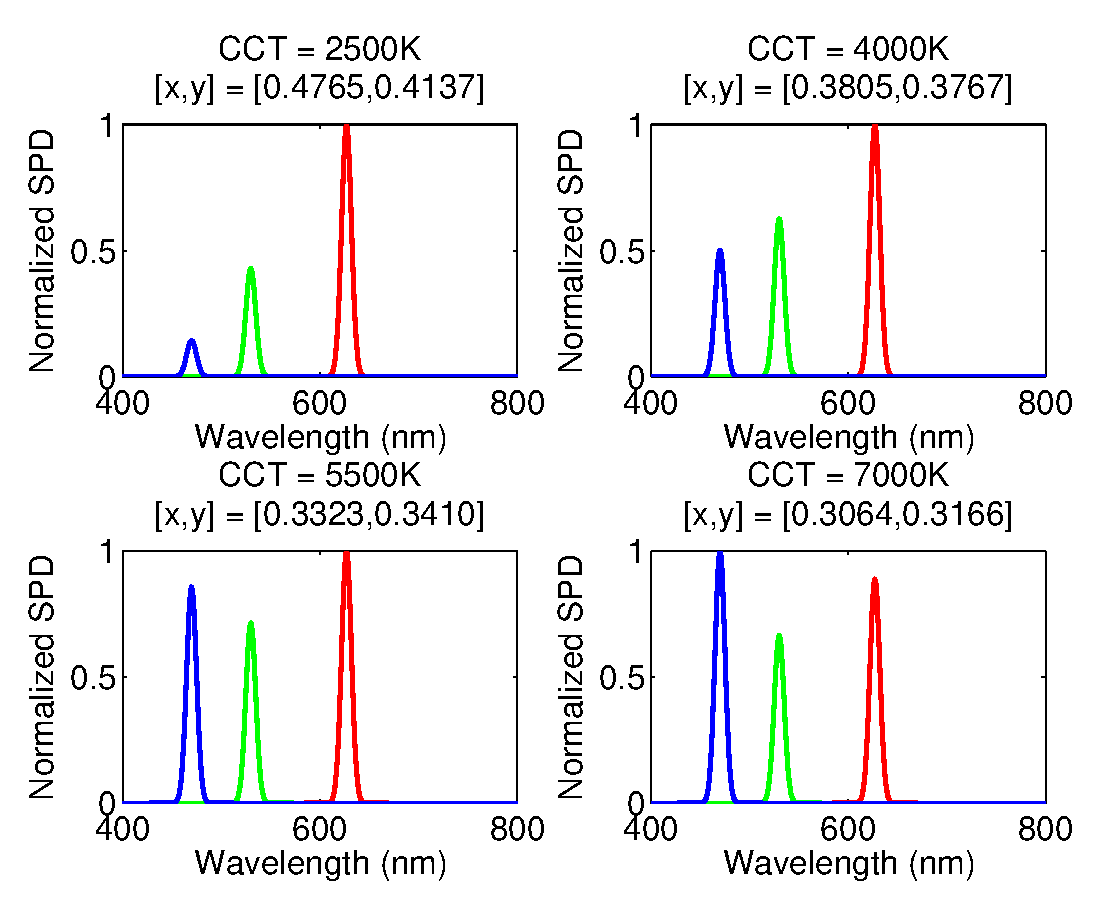
\includegraphics[width=3in]{img/LEDSPD.eps}
	\caption{Transmitting Element Normalized Spectral Power Distribution}
	\label{fig:LEDSPD}
\end{figure}

\begin{figure}
	\centering
		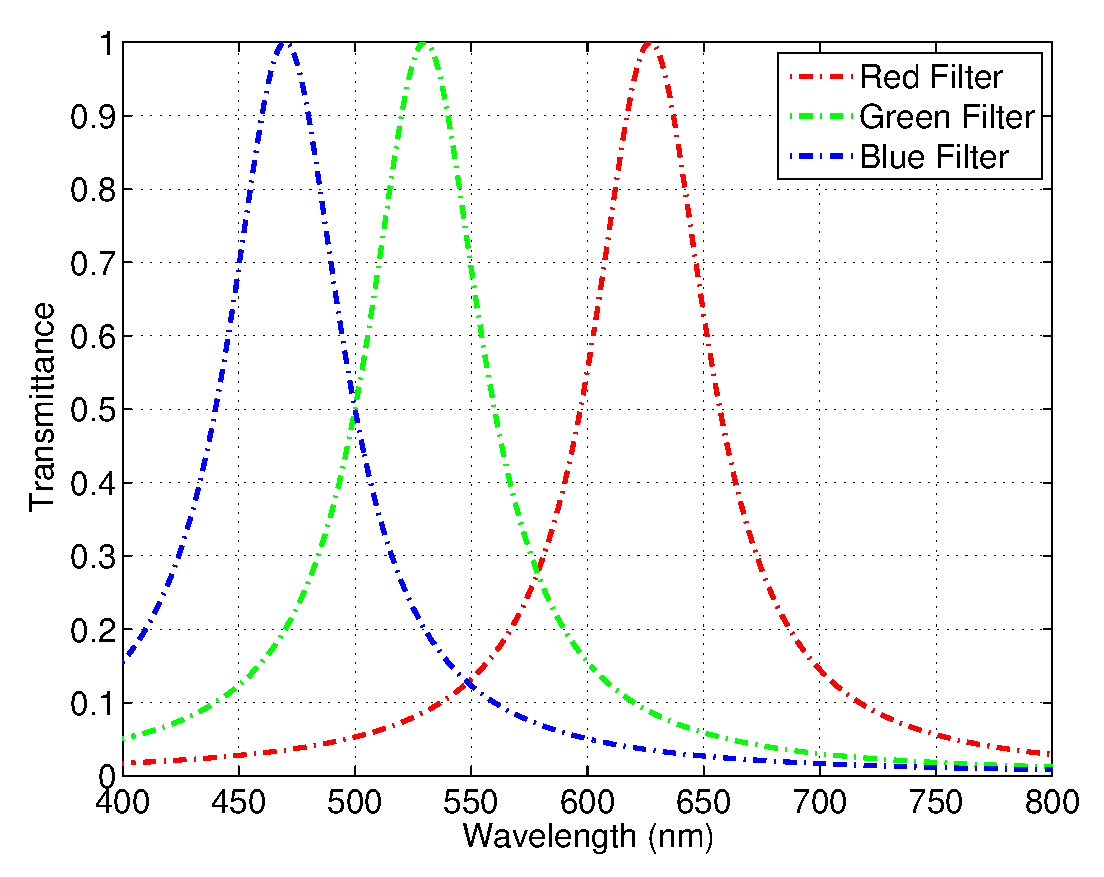
\includegraphics[width=3in]{img/FiltTr.eps}
	\caption{Filter Transmittance (FWHM=60nm)}
	\label{fig:FiltTr}
\end{figure}

\begin{figure}
	\centering
		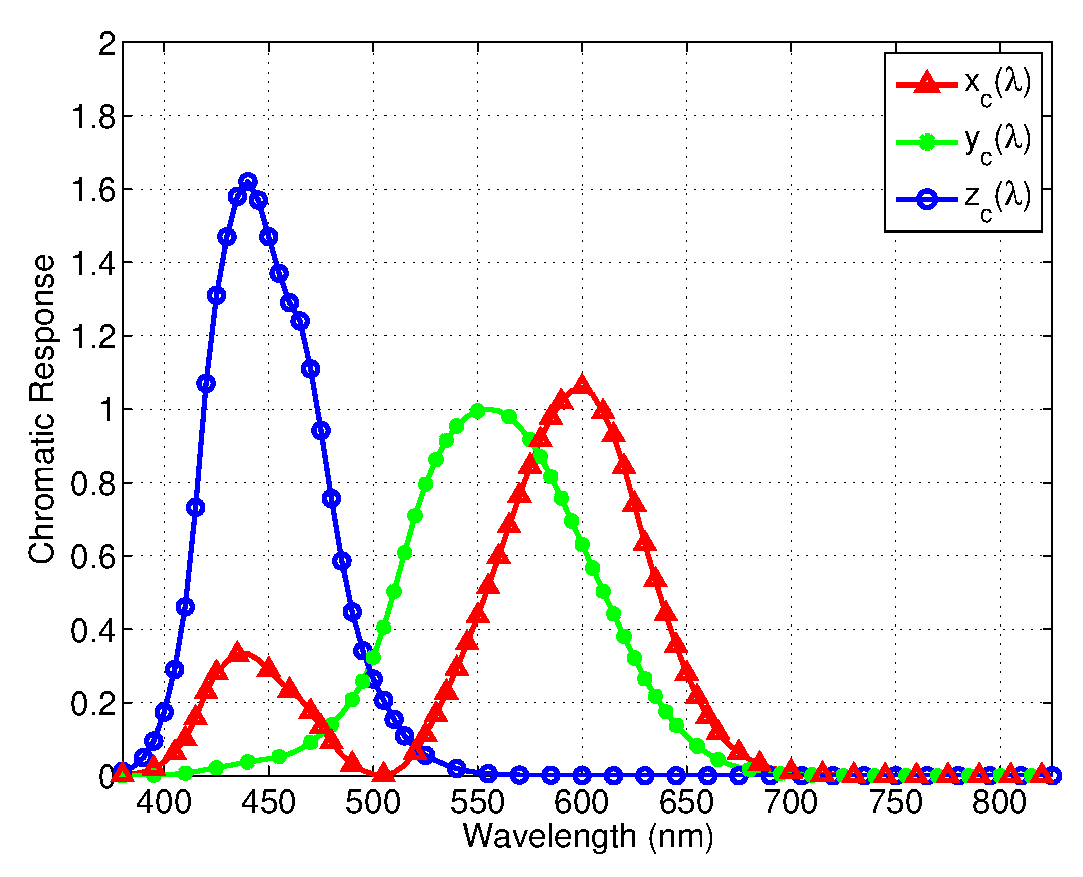
\includegraphics[width=3in]{img/CIE1931CMF.eps}
	\caption{CIE XYZ 1931 Model Color Matching Functions}
	\label{fig:CIE1931CMF}
\end{figure}

\begin{figure}
	\centering
		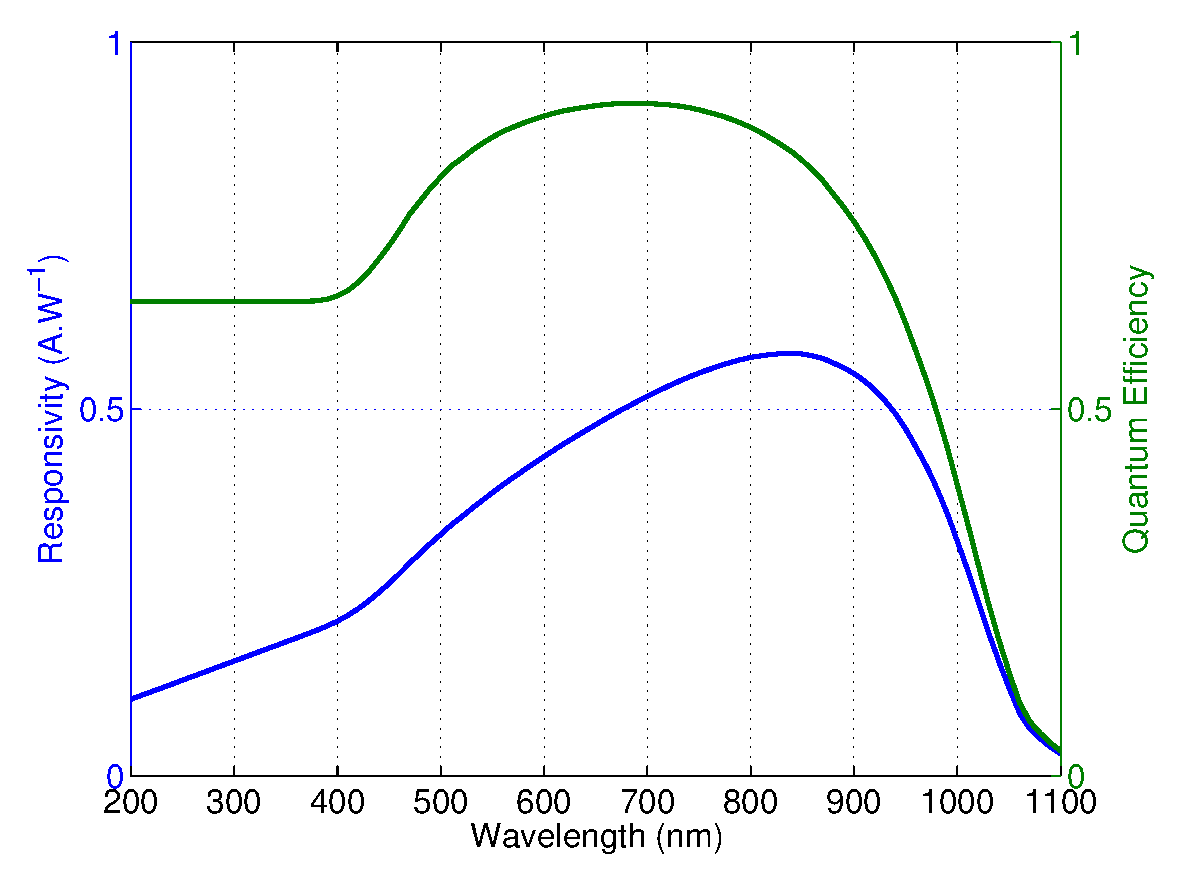
\includegraphics[width=3in]{img/RecvResp.eps}
	\caption{Receiver Responsivity}
	\label{fig:RecvResp}
\end{figure}

\begin{figure}
	\centering
		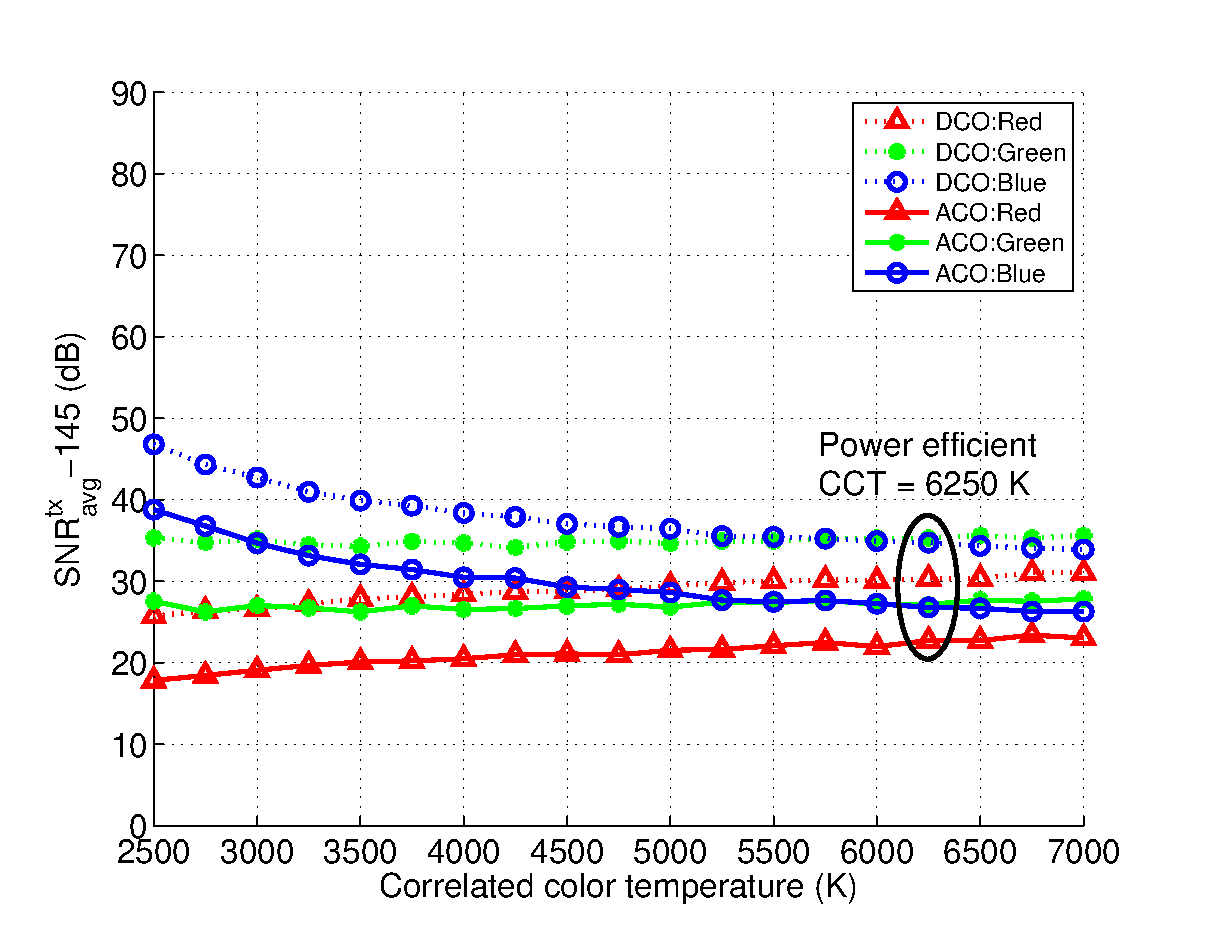
\includegraphics[width=3in]{img/SNRvsCCT.eps}
	\caption{$SNR_{avg}^{tx}$ vs Corelated Color Temperature}
	\label{fig:SNRvsCCT}
\end{figure}

\begin{figure}
	\centering
		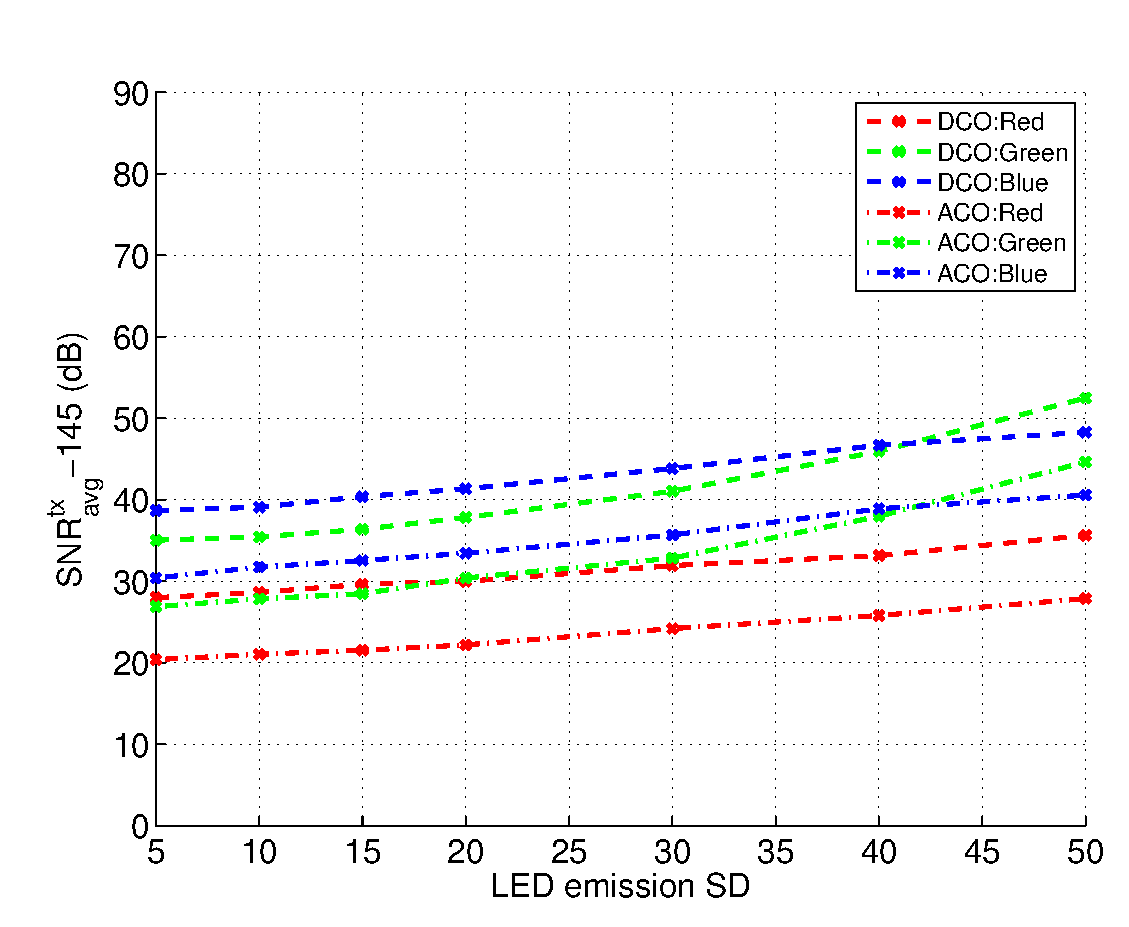
\includegraphics[width=3in]{img/SNRvsLEDSD.eps}
	\caption{$SNR_{avg}^{tx}$ vs Transmitting Element Spectral Power Distribution Width}
	\label{fig:SNRvsLEDSD}
\end{figure}

\begin{figure}
	\centering
		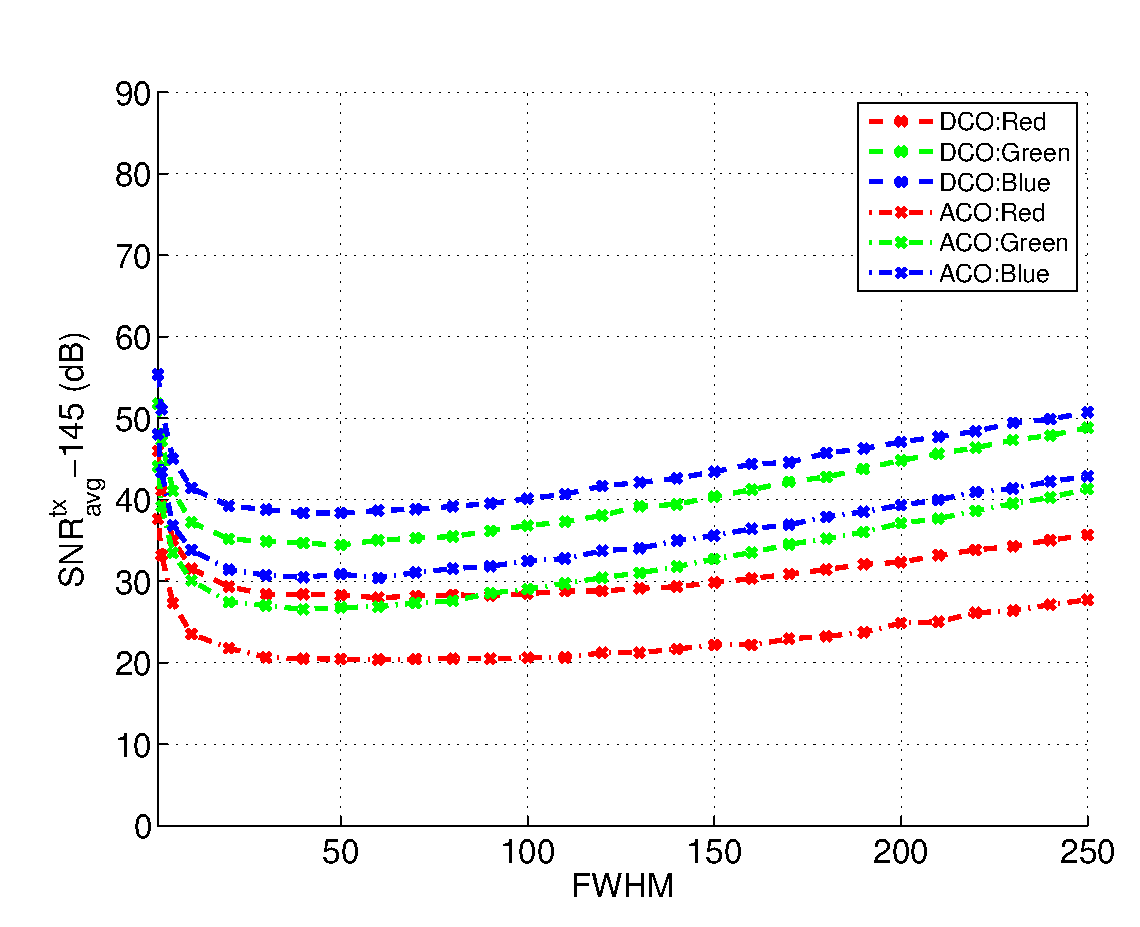
\includegraphics[width=3in]{img/SNRvsFLTWID.eps}
	\caption{$SNR_{avg}^{tx}$ vs Filter Full Width at Half Maximum}
	\label{fig:SNRvsFLTWID}
\end{figure}









